\documentclass[a4paper,11pt]{article}
\usepackage[margin=0.65in]{geometry}
\usepackage{booktabs}
\usepackage{amsmath}
\usepackage{hyperref}
\usepackage{float}
\usepackage{graphicx}
\usepackage{tabularx}
\usepackage{xcolor}
\usepackage{enumitem}
\usepackage{microtype}
\usepackage{titlesec}
\usepackage{fancyhdr}
\usepackage{lastpage}

\hypersetup{colorlinks=true,linkcolor=black,urlcolor=blue,citecolor=black}

\titleformat{\section}{\large\bfseries}{}{0pt}{}[\vspace{-0.3em}\rule{\textwidth}{0.5pt}]
\titleformat{\subsection}{\normalsize\bfseries}{}{0pt}{}
\titlespacing{\section}{0pt}{0.8em}{0.3em}
\titlespacing{\subsection}{0pt}{0.5em}{0.15em}

\setlength{\parindent}{0pt}
\setlength{\parskip}{0.2em}
\renewcommand{\arraystretch}{1.1}

\pagestyle{fancy}
\fancyhf{}
\renewcommand{\headrulewidth}{0.4pt}
\fancyhead[L]{\small AMCAS Assignment 1}
\fancyhead[R]{\small Abhinav Venkata Kota}
\fancyfoot[C]{\small\thepage\ / \pageref{LastPage}}

\begin{document}

\begin{center}
    {\Large\bfseries AMCAS Assignment 1}\\[0.5em]
    {\large Abhinav Venkata Kota}\\[0.1em]
    {\normalsize Roll No: 2024102059 \quad$\cdot$\quad IIIT Hyderabad ECE}
\end{center}

\vspace{0.3em}

%% ========================================================================
\section*{Part A -- ngspice: 6T SRAM Read Margin}
%% ========================================================================

\textit{Central question: does the bitcell read correctly at 0.7\,V and 85\,$^\circ$C?}

\begin{table}[H]
\centering
\small
\begin{tabularx}{\textwidth}{l X X}
\toprule
\textbf{Task} & \textbf{Result} & \textbf{Interpretation} \\
\midrule
1 & $\Delta V(BL,BLB)$ at 2\,ns = 729.86\,mV; $q_{\max}=205.52$\,mV. & Reads correctly; margin is ${\sim}10.6\times$ the 69\,mV lecture reference. \\[0.2em]
2 & Access width 0.24\,$\mu$m: $\Delta V=852.34$\,mV, $q_{\max}=271.22$\,mV. & Read disturb grows; cell is more marginal at worse PVT corners. \\[0.2em]
3 & $\Delta V$ falls below 25\,mV at $V_{DD}\approx0.448$\,V. & Within 1.1--0.6\,V sweep, read still safe; failure starts below ${\sim}0.45$\,V. \\[0.2em]
4 & At 85\,$^\circ$C: $\Delta V=582.12$\,mV, $q_{\max}=220.76$\,mV. & Limiting failure mode is read disturb, not sense-amp resolution. \\
\bottomrule
\end{tabularx}
\caption{Part A summary of nominal, sizing, supply, and temperature results.}
\end{table}

\subsection*{Task 1: Nominal Read Margin}

The bitline differential at $t=2$\,ns is 729.86\,mV ($q_{\max}=205.52$\,mV), giving ${\sim}10.6\times$ the 69\,mV sense-amp threshold. At nominal $V_{DD}=1.1$\,V the pull-down NMOS devices dominate the access transistors, keeping $v(Q)$ well below the inverter trip point.

\subsection*{Task 2: Access-Device Sizing}

Widening access transistors to 0.24\,$\mu$m increases $\Delta V$ to 852.34\,mV but raises $q_{\max}$ by 31.9\% to 271.22\,mV, degrading the $\beta$-ratio and eroding read stability. At worst-case PVT corners this reduced SNM could cause a destructive read.

\begin{figure}[H]
\centering
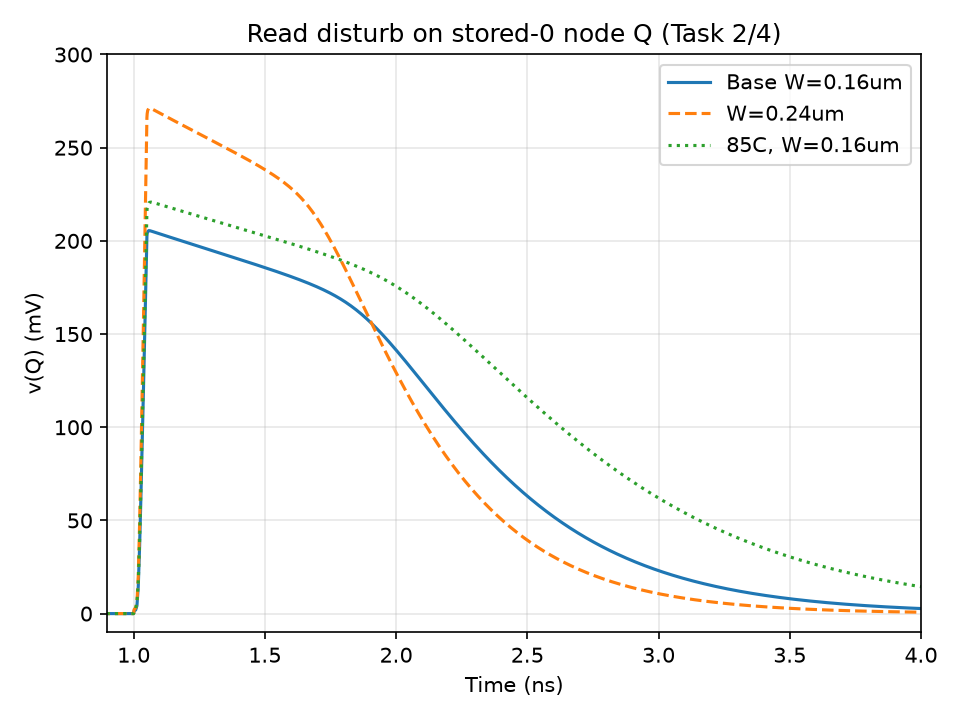
\includegraphics[width=0.78\textwidth]{../code_ngspice/Task-2_vq.png}
\caption{Read disturb $v(Q)$: nominal 205.5\,mV, widened access 271.2\,mV, 85\,$^\circ$C 220.8\,mV.}
\end{figure}

\subsection*{Task 3: Supply Sweep}

$\Delta V$ decreases monotonically with $V_{DD}$; the 25\,mV threshold is crossed at ${\approx}0.448$\,V (interpolated). Within 1.1--0.6\,V the minimum $\Delta V$ is 143.9\,mV (${\sim}5.8\times$ above threshold), so the read is safe across this range.

\begin{table}[H]
\centering
\footnotesize
\begin{tabularx}{\textwidth}{l *{6}{>{\centering\arraybackslash}X}}
\toprule
$V_{DD}$ (V) & 1.10 & 1.05 & 1.00 & 0.95 & 0.90 & 0.85 \\
$\Delta V$ (mV) & 729.9 & 673.6 & 616.0 & 557.1 & 497.4 & 437.2 \\
\midrule
$V_{DD}$ (V) & 0.80 & 0.75 & 0.70 & 0.65 & 0.60 & 0.55 \\
$\Delta V$ (mV) & 376.8 & 316.6 & 257.1 & 199.1 & 143.9 & 94.2 \\
\midrule
$V_{DD}$ (V) & 0.50 & 0.45 & 0.40 & & & \\
$\Delta V$ (mV) & 53.6 & 25.7 & 10.7 & & & \\
\bottomrule
\end{tabularx}
\caption{Part A Task 3 -- supply sweep. Interpolation between 0.45\,V and 0.40\,V gives the 25\,mV crossing near 0.448\,V.}
\end{table}

\begin{figure}[H]
\centering
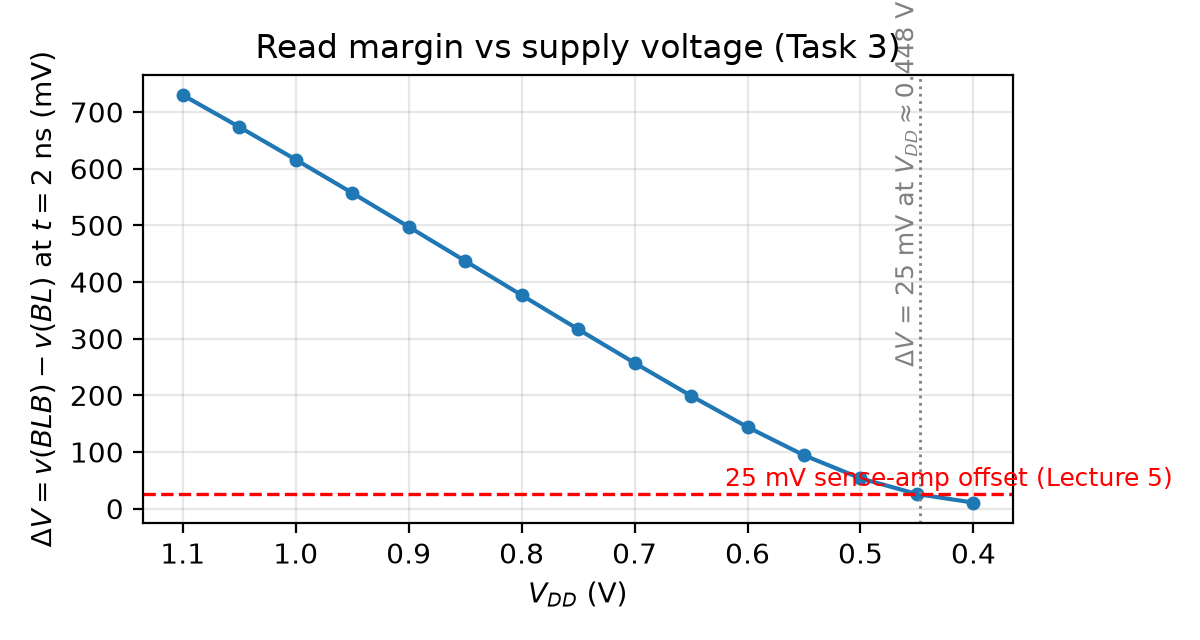
\includegraphics[width=0.78\textwidth]{../code_ngspice/Task-3_dv_vs_vdd.png}
\caption{$\Delta V$ at 2\,ns vs.\ $V_{DD}$; 25\,mV crossing near 0.448\,V, safe across 1.1--0.6\,V.}
\end{figure}

\subsection*{Task 4: Temperature Sensitivity}

At 85\,$^\circ$C, $\Delta V$ drops 20.2\% to 582.12\,mV and $q_{\max}$ rises 7.6\% to 220.76\,mV. Reduced carrier mobility lowers drive current while increased subthreshold leakage raises the stored-node disturbance, making read disturb the dominant high-temperature failure mechanism.

%% ========================================================================
\section*{Part B -- CACTI: 2\,MB SRAM L2}
%% ========================================================================

\textit{Central question: how fast, how big, and how leaky is a 2\,MB SRAM at 45\,nm?}

\subsection*{Task 1: Baseline Organization}

CACTI reports 2.90184\,ns access time, 0.792885\,nJ read energy, 562.632\,mW leakage, and 11.4742\,mm$^2$ area. The optimal organization is Ndwl/Ndbl/Nspd\,=\,4/2/1, balancing decoder delay, bitline length, wordline RC, and H-tree routing.

\subsection*{Task 2: Capacity Scaling}

\begin{table}[H]
\centering
\footnotesize
\begin{tabularx}{\textwidth}{l *{4}{>{\centering\arraybackslash}X}}
\toprule
\textbf{Capacity} & \textbf{Access (ns)} & \textbf{Read energy (nJ)} & \textbf{Leakage (mW)} & \textbf{Area (mm$^2$)} \\
\midrule
256\,kB  & 2.41714 & 0.658021 &   90.2876 &  4.96464 \\
512\,kB  & 2.48451 & 0.678967 &  158.126  &  5.94616 \\
1\,MB    & 2.63376 & 0.716643 &  293.680  &  7.59985 \\
2\,MB    & 2.90184 & 0.792885 &  562.632  & 11.4742  \\
4\,MB    & 3.53084 & 0.930134 & 1102.31   & 18.4579  \\
8\,MB    & 4.47269 & 1.21975  & 2183.82   & 39.4961  \\
16\,MB   & 6.36235 & 1.74213  & 4244.52   & 74.6677  \\
\bottomrule
\end{tabularx}
\caption{Part B Task 2 -- capacity sweep (256\,kB--16\,MB).}
\end{table}

\begin{figure}[H]
\centering
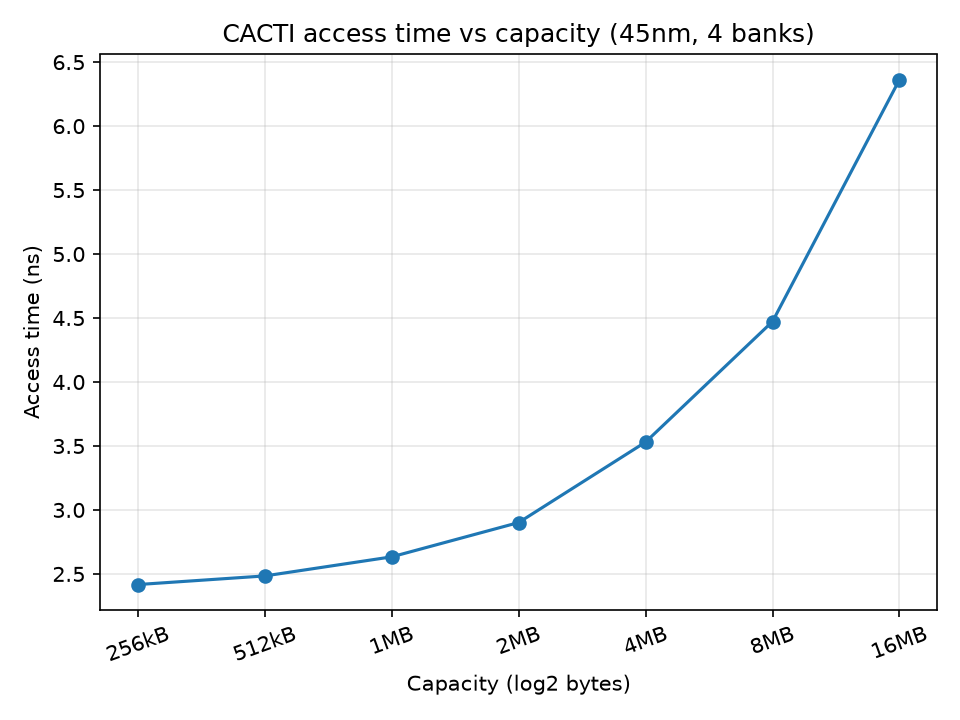
\includegraphics[width=0.78\textwidth]{../cacti/code_cacti/Task-2_capacity.png}
\caption{Access time vs.\ $\log_2$(capacity); linear to 2\,MB, super-linear after (H-tree RC dominates).}
\end{figure}

Access time grows $2.63\times$ for $64\times$ capacity (256\,kB$\rightarrow$16\,MB). Growth is super-linear at larger sizes because wire delay and H-tree routing dominate. Leakage and area scale near-linearly.

\subsection*{Task 3: Organization Objective}

\begin{table}[H]
\centering
\footnotesize
\begin{tabularx}{\textwidth}{l >{\centering\arraybackslash}X >{\centering\arraybackslash}X >{\centering\arraybackslash}X X}
\toprule
\textbf{Objective} & \textbf{Weight} & \textbf{Access (ns)} & \textbf{Ndwl/Ndbl/Nspd} & \textbf{Interpretation} \\
\midrule
Pure delay & 100:0:0:0:0 & 2.89231 & 4/2/1 & More mat parallelism minimizes critical path. \\
Pure area  & 0:0:0:0:100 & 3.35518 & 2/2/1 & Fewer subdivisions reduce peripheral overhead. \\
ED$^2$P    & 0:0:0:100:0 & 2.90184 & 4/2/1 & Delay benefit dominates energy--delay trade-off. \\
\bottomrule
\end{tabularx}
\caption{Part B Task 3 -- objective comparison (weight order: delay, dynamic energy, leakage, cycle time, area).}
\end{table}

Pure delay and ED$^2$P both select 4/2/1; pure area selects 2/2/1 with a 16\% access-time penalty. ED$^2$P agreeing with pure delay confirms delay reduction outweighs extra peripheral energy at this node.

\subsection*{Task 4: Bitline Delay Check}

CACTI reports a bitline delay of 0.4069\,ns; the lecture RC formula yields 18.7\,ns ($46\times$ overestimate). The discrepancy arises because the hand model assumes full-swing passive RC discharge, whereas the actual read is partial-swing (25--50\,mV) terminated early by the sense amplifier, and CACTI uses hierarchical bitline segments.

%% ========================================================================
\section*{Part C -- NVSim: 2\,MB STT-MRAM vs SRAM}
%% ========================================================================

\textit{Central question: same capacity, same periphery, different bitcell -- what changes?}

\begin{table}[H]
\centering
\small
\begin{tabularx}{\textwidth}{X >{\centering\arraybackslash}p{2.4cm} >{\centering\arraybackslash}p{2.4cm} >{\centering\arraybackslash}p{1.6cm}}
\toprule
\textbf{Metric} & \textbf{SRAM (CACTI)} & \textbf{STT-MRAM (NVSim)} & \textbf{Ratio} \\
\midrule
Area                & 11.474\,mm$^2$ & 3.590\,mm$^2$  & $0.31\times$ \\
Read hit latency    & 2.902\,ns      & 1.591\,ns      & $0.55\times$ \\
Write latency       & 2.902\,ns      & 10.608\,ns     & $3.66\times$ \\
Read energy         & 0.793\,nJ      & 0.763\,nJ      & $0.96\times$ \\
Write energy        & 0.851\,nJ      & 0.435\,nJ      & $0.51\times$ \\
Leakage power       & 562.6\,mW$^\dagger$ & 425\,mW     & $0.76\times$ \\
\bottomrule
\end{tabularx}
\caption{Part C Task 1 -- SRAM vs.\ STT-MRAM at 2\,MB, 45\,nm. $^\dagger$Cross-tool comparison (CACTI vs.\ NVSim). NVSim-internal SRAM reference: 6.393\,mm$^2$, 0.85/0.52\,ns, 3196\,mW; against that, STT-MRAM ratios are $0.56\times$ area, $1.87\times$/$20.4\times$ read/write latency, $0.13\times$ leakage.}
\end{table}

\subsection*{Task 1: SRAM--STT-MRAM Comparison}

STT-MRAM delivers $0.31\times$ area (1T-1MTJ at ${\sim}54$\,F$^2$ vs.\ SRAM's 146\,F$^2$) and $0.76\times$ leakage (magnetic storage needs no standby bias), but incurs a severe $3.66\times$ write penalty from spin-torque switching dynamics. These are cross-tool ratios; NVSim's own SRAM baseline confirms the expected $0.13\times$ leakage advantage.

\subsection*{Task 2: Strengths and Weaknesses}

\begin{table}[H]
\centering
\footnotesize
\begin{tabularx}{\textwidth}{l >{\centering\arraybackslash}X >{\centering\arraybackslash}X >{\centering\arraybackslash}X >{\centering\arraybackslash}X >{\centering\arraybackslash}X >{\centering\arraybackslash}X}
\toprule
\textbf{Config} & \textbf{Area} & \textbf{Rd lat.} & \textbf{Wr lat.} & \textbf{Rd E} & \textbf{Wr E} & \textbf{Leakage} \\
 & (mm$^2$) & (ns) & (ns) & (nJ) & (nJ) & (mW) \\
\midrule
SRAM baseline     & 6.393 & 0.850 &  0.520 & 0.575 & 0.531 & 3196.1 \\
STT-MRAM          & 3.590 & 1.591 & 10.608 & 0.763 & 0.435 &  425.2 \\
TMR high          & 3.580 & 1.596 & 10.657 & 0.761 & 0.433 &  425.2 \\
Half reset current & 3.590 & 1.571 & 10.588 & 0.762 & 0.433 &  425.0 \\
\bottomrule
\end{tabularx}
\caption{Part C Tasks 2--4 -- NVSim variants at 2\,MB, 45\,nm.}
\end{table}

Best STT-MRAM metrics: area ($0.56\times$), leakage ($0.13\times$), write energy ($0.82\times$). Worst: read latency ($1.87\times$), write latency ($20.4\times$), read energy ($1.33\times$).

\subsection*{Task 3: TMR Sensitivity}

Raising TMR from 2:1 to 3:1 produces negligible array-level changes (largest: write latency +0.46\%). TMR improves sense-amp signal margin and yield, not speed -- an important distinction for MRAM scaling.

\subsection*{Task 4: Write-Current Sensitivity}

Halving reset current (200$\rightarrow$100\,$\mu$A) does not change cell area (MTJ footprint dominates at 54\,F$^2$). Read latency drops $-$1.3\% and write energy $-$0.5\%. The primary STT-MRAM advantage is density and standby power, enabling ${\sim}4\times$ more capacity in the same area -- the key lever in Part~E.

%% ========================================================================
\section*{Part D -- Ramulator 2: DDR4 Miss Stream}
%% ========================================================================

\textit{Central question: how do scheduler, address mapping, and channel count change latency and throughput?}

\begin{table}[H]
\centering
\small
\begin{tabularx}{\textwidth}{X >{\centering\arraybackslash}p{1.5cm} >{\centering\arraybackslash}p{2.0cm} >{\centering\arraybackslash}p{1.8cm} >{\centering\arraybackslash}p{3.2cm}}
\toprule
\textbf{Configuration} & \textbf{Cycles} & \textbf{Avg read lat.} & \textbf{Row-hit rate} & \textbf{Note} \\
\midrule
FRFCFS + RoBaRaCoCh    & 9\,594  & 262.93  & 53.9\% & Baseline \\
FCFS-proxy (buf=1)     & 42\,937 & 61.90   & 69.6\% & No reordering; much slower \\
ChRaBaRoCo             & 78\,845 & 1844.21 & 55.9\% & Row locality destroyed \\
2 channels             & 4\,889  & 233.57  & 32.7\% & Best throughput \\
\bottomrule
\end{tabularx}
\caption{Part D -- scheduler, address-mapping, and channel comparison (2\,048-request trace).}
\end{table}

\subsection*{Task 1: Baseline Scheduler and Mapping}

With FRFCFS and RoBaRaCoCh the trace completes in 9\,594 cycles (262.93 avg read latency, 53.9\% row-hit rate). FRFCFS prioritizes row-buffer hits, and RoBaRaCoCh maps consecutive addresses to columns within the same row.

\begin{table}[H]
\centering
\footnotesize
\begin{tabularx}{\textwidth}{X >{\centering\arraybackslash}p{1.4cm} >{\centering\arraybackslash}p{1.6cm} >{\centering\arraybackslash}p{1.2cm} >{\centering\arraybackslash}p{1.2cm} >{\centering\arraybackslash}p{1.4cm} >{\centering\arraybackslash}p{1.3cm}}
\toprule
\textbf{Configuration} & \textbf{Cycles} & \textbf{Read lat.} & \textbf{Hits} & \textbf{Misses} & \textbf{Conflicts} & \textbf{Hit rate} \\
\midrule
FRFCFS + RoBaRaCoCh & 9\,594  & 262.93  & 1\,079 & 215 & 707 & 53.9\% \\
FCFS proxy          & 42\,937 & 61.90   & --     & --  & --  & 69.6\% \\
ChRaBaRoCo          & 78\,845 & 1844.21 & 1\,121 &   7 & 878 & 55.9\% \\
2 channels          & 4\,889  & 233.57  &   326  & 143 & 528 & 32.7\% \\
\bottomrule
\end{tabularx}
\caption{Part D -- row-buffer breakdown across configurations.}
\end{table}

\subsection*{Task 2: Scheduler Comparison}

The FCFS-proxy achieves higher row-hit rate (69.6\%) but $4.5\times$ worse throughput (42\,937 cycles), demonstrating that bank-level parallelism and request reordering matter more than raw hit rate. FRFCFS prioritizes requests that hit an already-open row (``first-ready'') over older requests stalled on timing, so it overlaps precharge--activate sequences on one bank with data bursts on another. With tRCD = tRP = 22 cycles, every row conflict costs a 44-cycle precharge--activate round trip before the column command can issue; FCFS pays this serially on the critical path, while FRFCFS hides it behind useful work on idle banks. The proxy's buffer depth of 1 additionally serializes issue (no queue to pick from), turning every timing constraint into a stall. Its lower per-request latency (61.90 cycles) is therefore an artifact of an unloaded, non-reordering model rather than a genuine advantage -- throughput, not single-request latency, is the scheduler's job.

\subsection*{Task 3: Address Mapping}

ChRaBaRoCo is catastrophic (78\,845 cycles, $8.2\times$ baseline): placing row bits below bank bits maps consecutive cache-line addresses to different rows in the same bank, converting most accesses to costly conflicts (878 vs.\ 707 baseline, misses collapsing to 7). Each conflict pays the full tRP + tRCD penalty plus queueing behind the bank's busy row, and average read latency explodes to 1844.21 cycles. The row-hit rate barely moves (55.9\% vs.\ 53.9\%) because the few remaining hits are accidental, while bank-level parallelism -- the mechanism FRFCFS relies on -- is destroyed: with consecutive lines colliding in one bank, the scheduler finds no ready request elsewhere while that bank grinds through precharge--activate. This is why address mapping is a first-order memory-controller decision: RoBaRaCoCh stripes sequential lines across columns of one row (hits) and across banks (parallelism), whereas row-below-bank concentrates them into conflicts.

\subsection*{Task 4: Channels and Timing Sensitivity}

A second channel cuts cycles nearly in half (4\,889, $1.96\times$ speedup) despite lower row-hit rate (32.7\%): channel interleaving splits spatially local lines across two independent controllers, halving per-channel locality but doubling service bandwidth. Throughput scales because the two channels retire requests concurrently; per-request latency barely improves (233.57 vs.\ 262.93 cycles, $-11\%$) since a single access still pays the same DRAM timing. This throughput-vs-latency split is the expected signature of channel scaling and confirms the trace is bandwidth-bound rather than latency-bound.

\begin{table}[H]
\centering
\small
\begin{tabularx}{\textwidth}{X >{\centering\arraybackslash}p{2.5cm} >{\centering\arraybackslash}p{2.5cm} >{\centering\arraybackslash}p{3cm}}
\toprule
\textbf{Timing parameter} & \textbf{Cycles} & \textbf{Avg read lat.} & \textbf{Increase from baseline} \\
\midrule
Baseline                    & 9\,594  & 262.9 & -- \\
tRCD: 22 $\rightarrow$ 44  & 10\,534 & 291.9 & +9.8\% \\
tRP: 22 $\rightarrow$ 44   & 10\,625 & 281.9 & +10.7\% \\
tRAS: 52 $\rightarrow$ 104 & 10\,003 & 269.0 & +4.3\% \\
tCCD: 4 $\rightarrow$ 8    & 12\,203 & 322.1 & +27.2\% \\
\bottomrule
\end{tabularx}
\caption{Part D Task 4 -- timing-sensitivity experiment.}
\end{table}

tCCD is the binding constraint (+27.2\%), far exceeding tRCD/tRP/tRAS, because the 53.9\% hit rate means many accesses are gated only by column-to-column spacing within an open row. Doubling tRCD or tRP (+9.8\%/+10.7\%) hurts only the conflict/miss fraction, and tRAS (+4.3\%) rarely binds since rows stay open across multiple column hits. The way to determine this from the output is the single-parameter sweep in the table: vary one timing knob at a time with trace, scheduler, and mapping fixed, then rank by cycles increase. The knob whose doubling moves total cycles most is binding for that workload; here tCCD's 27.2\% dominates because this trace is row-locality rich. A conflict-heavy trace (e.g.\ ChRaBaRoCo) would instead crown tRP/tRCD -- binding is a property of workload $\times$ mapping, not of the DRAM alone. For the central question, Part~D's lesson is that every L2 miss that reaches DRAM costs hundreds of cycles and its price depends on scheduler, mapping, and channel count; Part~E's miss-rate deltas must therefore be read through this backend cost, which is exactly what makes the 8\,MB MRAM capacity win at \texttt{-g\,14}.

%% ========================================================================
\section*{Part E -- gem5: Whole-Program Simulation}
%% ========================================================================

\textit{Central question: does the program you care about actually run faster with STT-MRAM?}

Part B gives SRAM a 7-cycle L2 hit latency (2.90\,ns at ${\sim}2$\,GHz); Part~C shows the same die area holds ${\sim}8$\,MB of STT-MRAM at 14-cycle hit latency. gem5 compares 2\,MB/7-cycle SRAM vs.\ 8\,MB/14-cycle STT-MRAM at \texttt{-g\,14} (O3CPU) and \texttt{-g\,10} (TimingSimpleCPU).

\begin{table}[H]
\centering
\small
\begin{tabularx}{\textwidth}{X >{\centering\arraybackslash}p{1.4cm} >{\centering\arraybackslash}p{2.0cm} >{\centering\arraybackslash}p{2.0cm} >{\centering\arraybackslash}p{2.8cm}}
\toprule
\textbf{Kernel / Config} & \textbf{IPC} & \textbf{L2 miss rate} & \textbf{simSeconds} & \textbf{simInsts} \\
\midrule
bfs\,/\,SRAM (2\,MB, 7\,cyc)   & 0.3335 & 16.64\% & 0.43711 & 291\,572\,930 \\
bfs\,/\,MRAM (8\,MB, 14\,cyc)  & 0.3392 & 7.78\%  & 0.42985 & 291\,572\,930 \\
sssp\,/\,SRAM (2\,MB, 7\,cyc)  & 0.3158 & 31.46\% & 0.54299 & 342\,904\,674 \\
sssp\,/\,MRAM (8\,MB, 14\,cyc) & 0.3313 & 9.50\%  & 0.51754 & 342\,904\,674 \\
\bottomrule
\end{tabularx}
\caption{Part E Task 1 -- gem5 O3CPU comparison at \texttt{-g\,14}.}
\label{tab:partE}
\end{table}

\subsection*{Task 1: Whole-Program Comparison}

STT-MRAM wins on both kernels (bfs $1.017\times$, sssp $1.049\times$). Miss rates drop substantially (16.64\%$\rightarrow$7.78\% bfs, 31.46\%$\rightarrow$9.50\% sssp); each avoided miss saves ${\sim}100$+ DRAM cycles vs.\ only 7 extra cycles per hit.

\begin{table}[H]
\centering
\footnotesize
\begin{tabularx}{\textwidth}{l >{\centering\arraybackslash}X >{\centering\arraybackslash}X >{\centering\arraybackslash}X X}
\toprule
\textbf{Kernel (TimingSimple, -g\,10)} & \textbf{SRAM simS} & \textbf{MRAM simS} & \textbf{L2 miss rate} & \textbf{Winner} \\
\midrule
bfs  & 0.020957 & 0.020972 & 27.85\% $\rightarrow$ 27.85\% & SRAM (+0.07\%) \\
sssp & 0.027119 & 0.027146 & 25.11\% $\rightarrow$ 25.11\% & SRAM (+0.10\%) \\
\bottomrule
\end{tabularx}
\caption{Part E -- scale sensitivity at \texttt{-g\,10}: working set fits in both caches, so capacity buys nothing and latency decides.}
\end{table}

\subsection*{Task 2: Kernel Sensitivity}

sssp benefits ${\sim}3\times$ more (4.9\% vs.\ 1.7\%) because its 2\,MB miss rate (31.46\%) is much higher than bfs (16.64\%), so the extra capacity captures proportionally more of its working set. The breakeven arithmetic favors capacity heavily here: each avoided L2 miss saves a full DRAM round trip (${\sim}100$+ cycles per Part~D's latency analysis), while each retained hit pays only 7 extra cycles ($14-7$). For sssp, the miss count falls by roughly $70\%$, converting tens of thousands of DRAM accesses into L2 hits; the 7-cycle tax on hits is an order of magnitude smaller than the saved miss penalty, hence the 4.9\% net win. For bfs, the working set already partially fits in 2\,MB (16.64\% miss), so the same $4\times$ capacity buys a smaller absolute miss reduction ($-53\%$ relatively, but from a lower base) and the net is only 1.7\%. This is the general principle the assignment targets: capacity upgrades pay off in proportion to the baseline miss rate, and pointer-chasing graph kernels with poor locality (sssp's frontier expansion over irregular edges) sit exactly in the regime where density beats latency.

\subsection*{Task 3: CPU-Model Effect}

The O3CPU partially hides MRAM's $2\times$ hit-latency penalty by overlapping independent work during stalls. A TimingSimpleCPU exposes every stall directly, making the measured 1.7--4.9\% MRAM advantage conservative for in-order cores. The \texttt{-g\,10} TimingSimple sweep confirms the mechanism from the other side: with identical miss rates across cache sizes (27.85\% bfs, 25.11\% sssp -- capacity buys nothing), the in-order core reports SRAM faster by exactly the hit-latency delta (+0.07\% bfs, +0.10\% sssp), since every L2 hit costs 7 extra cycles under MRAM with no avoided DRAM access to compensate. In other words, the CPU model sets the exchange rate between hits and misses: out-of-order execution discounts the per-hit tax (favoring MRAM at \texttt{-g\,14}), while in-order execution charges it in full (which is why the \texttt{-g\,10} SRAM margin, though tiny in absolute terms, is structurally pure latency). Any cross-core comparison must therefore normalize by this effect before attributing deltas to the memory technology itself.

\subsection*{Task 4: Final System Choice}

\begin{table}[H]
\centering
\small
\begin{tabularx}{\textwidth}{l X X}
\toprule
\textbf{Task} & \textbf{Result} & \textbf{Reasoning} \\
\midrule
2 & MRAM wins at \texttt{-g\,14}; sssp benefits more. & Poorer locality gains more from capacity. \\[0.2em]
3 & O3 hides part of cache-stall cost. & In-order core exposes stalls directly. \\[0.2em]
4 & MRAM wins at \texttt{-g\,14}, SRAM at \texttt{-g\,10}; predicted SRAM at \texttt{-g\,18}. & Below 2\,MB latency decides; at 2--8\,MB capacity decides; beyond 8\,MB both miss alike. \\
\bottomrule
\end{tabularx}
\caption{Part E Tasks 2--4 -- interpretation summary.}
\end{table}

STT-MRAM is preferred at \texttt{-g\,14}: the miss-rate reduction ($-53\%$ bfs, $-70\%$ sssp) outweighs the $2\times$ hit-latency penalty. Caveats: (i)~the $4\times$ capacity ratio may be optimistic if peripherals do not scale; (ii)~\texttt{-g\,18} was not run -- overflowing both caches would equalize miss rates, letting the latency penalty dominate. The MRAM advantage is scale-dependent.

%% ========================================================================
\section*{Conclusion}
%% ========================================================================

SRAM is faster per-access, but STT-MRAM wins at the system level when its ${\sim}4\times$ density converts to large miss-rate reduction (\texttt{-g\,14}: +1.7--4.9\%). When the working set fits both caches (\texttt{-g\,10}) or overflows both (predicted \texttt{-g\,18}), SRAM's $2\times$ faster hits win. Device speed alone does not decide; workload locality, DRAM policy, and CPU model tilt the balance. Code: \url{https://github.com/DevAbhinav-23/AMCAS_Assignments}.

\end{document}